\label{sec:NuMUCCsel}

\par This chapter presents the two $\nu_{\mu}$ selections of the analysis; both are inclusive selections, but with different distributions. The first selection (sec \ref{ssec:NuMUCCsel:INC}) provides a pure, high-statistics sample of $\nu_{\mu}$s and the second selection (sec \ref{ssec:NuMUCCsel:constr}) is optimized to be used as a constraining tool in the $\nu_e$ analysis \textcolor{blue}{with a particular emphasis on reconstructing low-energy neutrino interactions}. 
\textcolor{blue}{The inclusive selection of Sec.~\ref{ssec:NuMUCCsel:INC} is particularly well suited as a filter for multiple exclusive channel measurements, which, while not currently performed and included in this analysis, may provide helpful and necessary validations and constraints on neutrino interaction modeling as the analysis matures in the coming months.}

\subsection{Variable Definitions}
\label{ssec:NuMUCCsel:sel:vars}

\par Table~\ref{tab:numuvariableSummary} contains a concise list of variables used in the $\nu_{\mu}$ selections. The variables are organized into \textit{slice} and \textit{track}-level descriptors, used for preselection and muon-candidate selection respectively. There is some redundancy between this list and the list in sec \ref{sec:nueselection:variables}, but this list below should serve as a quick reference to a reader of this chapter.

\begin{table}[ht]
\caption{\label{tab:numuvariableSummary} Summary of the definition for the variables used in the $\nu_{\mu}$ selections.}
\centering
\begin{tabular}{ m{0.08\textwidth} | m{0.25\textwidth} | m{0.55\textwidth}  }
Category & Variable Name & Description  \\
\hline

\multicolumn{1}{l|}{} & \emph{nslice} &  Number of neutrino slices identified by the \emph{SliceID}. Values are  0 or 1.\\  \cline{2-3}
\multicolumn{1}{l|}{} & \emph{slpdg} &  PDG code of the event as assigned by Pandora, 12 if the object with the most hits over all planes is shower-like, 14 if track-like.\\  \cline{2-3}
\multicolumn{1}{l|}{} & \emph{all\_\{start,end\}\_contained} &  The start/end points of all PFParticles are volume defined with borders: \SI{5}{\cm} in $x$ and \SI{6}{\cm} $y$ and \SI{10}{\cm} $z$.\\  \cline{2-3}
\multicolumn{1}{l|}{} & \emph{slpdg} &  PDG code of the event as assigned by Pandora, 12 if the object with the most hits over all planes is shower-like, 14 if track-like.\\  \cline{2-3}
\multicolumn{1}{l|}{} & \emph{n\_tracks\_contained} &  number of tracks fully contained in the fiducial volume.\\  \cline{2-3}
\multicolumn{1}{l|}{} & \emph{reco\_nu\_vtx\_sce\_\{x,y,z\}} & Reconstructed neutrino interaction vertex in (x,y,z) coordinates. The space charged correction is applied.  \\  \cline{2-3}
\parbox[t]{2mm}{\multirow{4}{*}{\rotatebox[origin=c]{90}{Slice}}} & \emph{hits\_ratio} & Ratio between hits from showers and total number of hits in the slice. \\  \cline{2-3}
\multicolumn{1}{l|}{} & \emph{CosmicIP} & Closest distance between shower start and space points associated to tracks flagged as cosmics. \\  \cline{2-3}
\multicolumn{1}{l|}{} & \emph{crtveto} & Boolean variable checking if the event passes the CRT veto. \\  \cline{2-3}
\multicolumn{1}{l|}{} & \emph{\_closestNuCosmicDist} &  3D distance between the reconstructed neutrino vertex and the closest CRT-tagged cosmic track. \\  \cline{2-3}
\hline


\multicolumn{1}{l|}{} & \emph{trk\_sce\_\{start,end\}\_\{x,y,z\}} &  Reconstructed, spacecharge-corrected start/end-points for the tracks.\\  \cline{2-3}
\multicolumn{1}{l|}{} & \emph{trk\_llr\_pid\_score} &  The log likelihood ratio particle identification score (see sec. \ref{subsec:loglikelihoodpid}). This variable has strong muon-proton discriminating power (see fig. \ref{fig:numu:topo_pid}).\\  \cline{2-3}
\multicolumn{1}{l|}{} & \emph{trk\_score} & A machine-learned quantity that describes how `track-like' the reconstructed object is (possible values between 0 and 1). \\  \cline{2-3}
\parbox[t]{2mm}{\multirow{4}{*}{\rotatebox[origin=c]{90}{Track}}} & \emph{trk\_len} & he length of the reconstructed track (in cm). \\  \cline{2-3}
\multicolumn{1}{l|}{} & \emph{trk\_distance} & The distance from the start-point of the reconstructed track to the reconstructed neutrino vertex (in cm). \\  \cline{2-3}
\multicolumn{1}{l|}{} & \emph{pfp\_generation} &  The generation of the PFParticle according to Pandora: the neutrino has generation 1, it's direct daughters 2, and further decay products 3 or higher.\\  \cline{2-3}
\hline

\end{tabular}
\label{tab:numuvariableSummary}
\end{table}

\begin{comment}

\par \noindent \textbf{Slice variables}: These variables generally describe the reconstructed neutrino interaction, i.e. the confluence of data gathered from all the PFParticles in the slice.
\begin{itemize}
    \item \emph{nslice}: number of neutrino slices identified by the SliceID (possible values are 0 or 1).
    \item \emph{n\_tracks\_contained}: number of tracks fully contained in the fiducial volume.
    \item \emph{reco\_nu\_vtx\_sce\_\{x,y,z\}}: Reconstructed, spacecharge-corrected neutrino interaction vertices in (x,y,z) coordinates (see fig. \ref{fig:numu_vtx}.
    \item \emph{topological\_score}: A machine-learned quantity that reflects the complexity and directionality of observable slice quantities. This variable has strong discriminating power between signal and cosmic-background (see \ref{fig:numu_topo_pid} (possible values are between 0 and 1).
    \item \emph{CRT Veto and Distance Tagger}: Tools provided by the cosmic ray tagger (see sec. \ref{sec:sliceID:CRT}).
\end{itemize}

\par \noindent \textbf{Track variables}: These variables specifically describe the reconstructed PFParticles; in interest to this selection are reconstructed track-like objects. 
\begin{itemize}
    \item \emph{trk\_sce\_\{start,end\}\_\{x,y,z\}}: Reconstructed, spacecharge-corrected start/end-points for the tracks.
    \item \emph{trk\_llr\_pid\_score}: The log likelihood ratio particle identification score (see sec. \ref{subsec:loglikelihoodpid}). This variable has strong muon-proton discriminating power (see fig. \ref{fig:numu_topo_pid}).
    \item \emph{trk\_score}: A machine-learned quantity that describes how `track-like' the reconstructed object is (possible values between 0 and 1).
    \item \emph{trk\_len}: The length of the reconstructed track (in cm).
    \item \emph{trk\_distance}: The distance from the start-point of the reconstructed track to the reconstructed neutrino vertex (in cm).
    \item \emph{pfp\_generation}: The generation of the PFParticle according to Pandora, i.e. the neutrino has generation 1, its direct daughters generation 2 and further decay products have generation 3.
\end{itemize}
\end{comment}

\begin{comment}
\subsubsection{Backgrounds}
\label{sssec:NuMUCCsel:sel:bkgrnds}

\par Coming soon...

\subsubsection{Fiducial Volume and Spacecharge-Corrected Spacepoints}
\label{sssec:NuMUCCsel:sel:FVandSCE}

\par Coming soon...
\end{comment}



\subsection{Inclusive Selection}
\label{ssec:NuMUCCsel:INC}
The $\nu_\mu$ CC Inclusive selection is an update from the selection that is currently be used as a filter and described in an internal note~\cite{bib:numuccfilter}. This selection aims to be as similar as possible to the $\nu_e$ CC Inclusive selection described in \cref{sec:nueselection:inclusive}, with the ultimate goal to perform a $\nu_\mu$ constrained BNB electron neutrino measurement. 

\paragraph{$\nu_\mu$ CC inclusive signal definition}
\begin{itemize}
    \item One final state muon with a kinetic energy above \SI{20}{\MeV}.
    \item True neutrino vertex inside a fiducial volume defined with borders: \SI{10}{\cm} in $x$ and $y$ and $[ \SI{20}{\cm}, \SI{50}{\cm}]$ in $z$.
\end{itemize}
The cut on the true energy corresponds to a track length of \SI{\approx 2.5}{\cm}.

\paragraph{Event selection}
Before identifying the muon, some event level cuts are applied:

\begin{itemize}
    \item \textit{slpdg= 14}
    \item \textit{CosmicIP} $>$ \SI{20}{\cm}
    \item \textit{topological\_score $>$ 0.1}
    \item \textit{all\_start\_contained}
\end{itemize} 

The next step is to identify a muon track.
\paragraph{Muon candidate identification} 
\begin{itemize}
    \item \textit{trk\_score $>$ 0.8}
    \item \textit{trk\_len} $>$ \SI{10}{\cm}
    \item \textit{trk\_llr\_pid\_score $>$ 0.2}
    \item \textit{pfp\_generation = 2}
    \item \textit{trk\_distance} $<$ \SI{4}{\cm}
\end{itemize}
At this point, the amount of muon candidate tracks in signal events is:
\begin{itemize}
    \item 0 (10\%), the event gets rejected.
    \item 1 (70\%), the event gets selected.
    \item 2 (18\%) or $>2$ (2\%), the particle with the highest \textit{trk\_llr\_pid\_score} is picked as muon and the event is selected.
\end{itemize}

The cut on the reconstructed length corresponds to a muon kinetic energy of \SI{\approx 47}{\MeV} kinetic energy or a muon momentum of \SI{0.11}{GeV/c}. Therefore, this selection aim to have a lower neutrino energy threshold of \SI{\approx 153}{\MeV}. Therefore, efficiency plots will be shown in a range from \SIrange{0.15}{1.65}{\GeV} in this section.

\begin{figure}
    \centering
    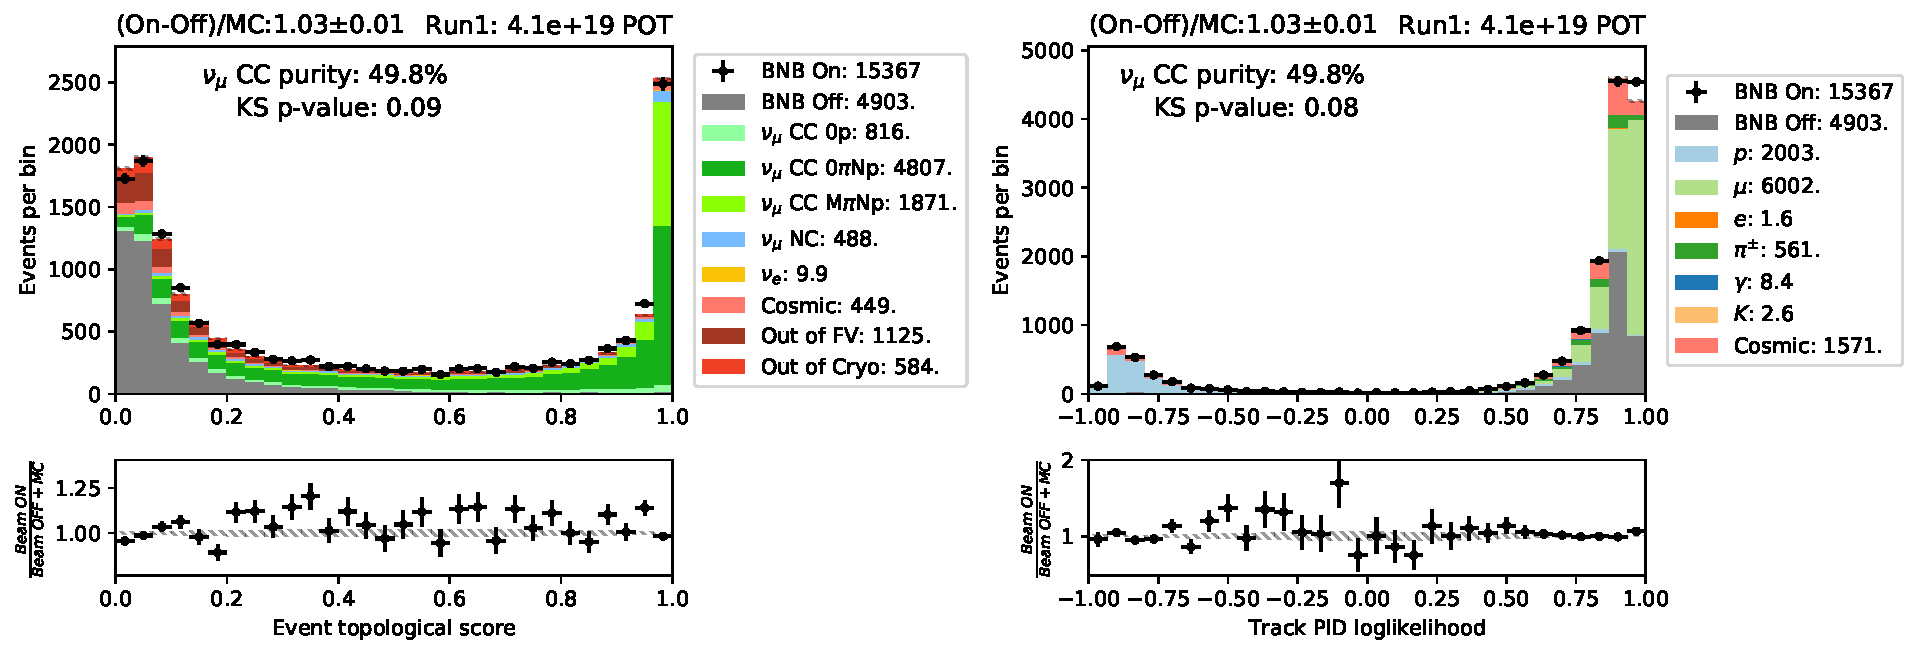
\includegraphics[width=\textwidth]{NuMuCCsel/Images/run1/numu_pret_run1.pdf}
    \caption{Topological score and track PID likelihood distributions after all other cuts are applied in the $\nu_\mu$ CC inclusive selection.}
    \label{fig:numu:topo_pid}
\end{figure}

The distribution of the topological score and the track muon likelihood after applying all cuts except these two is given in \cref{fig:numu:topo_pid}.

\paragraph{Event selection performance}

\begin{figure}[H]
    \centering
    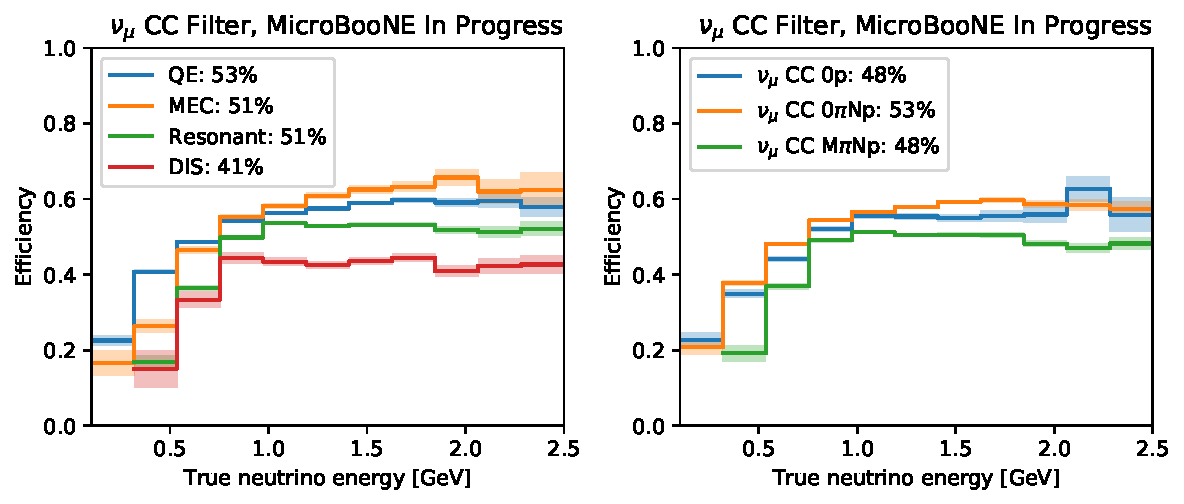
\includegraphics[width=0.65\textwidth]{NuMuCCsel/Images/run1/numu_efficiency_run1.pdf}
    \caption{Efficiency of the $\nu_\mu$ CC inclusive selection for different interaction categories (left) and final states (right) in function of the true neutrino energy. }
    \label{fig:numu:eff_r1}
\end{figure}

\cref{fig:numu:eff_r1} shows the efficiency in function of the true neutrino energy, integrated over all energies for all singal event categories, the efficiency is 51.1\%. It can be seen that the selection is truly inclusive in both interaction type and final states. non-zero efficiencies are reached from \SI{150}{\MeV} and the efficiency flattens out at \SI{\approx 700}{\MeV}. The overall purity of the selection is 65.9\% with the in-time cosmic activity as dominant background. In 94.7\% of the events, the track identified as muon is backtracked to the muon correctly. Most mis-identification cases correspond to charged pions (3.6\%).

Because this selection contains both contained and uncontained events, multiple coulomb scattering is used to measure the muon momentum. \cref{fig:numu:mcs,fig:numu:vtx} show the muon candidate kinematics and the reconstructed vertex position after selection.


\begin{figure}[H]
    \centering
    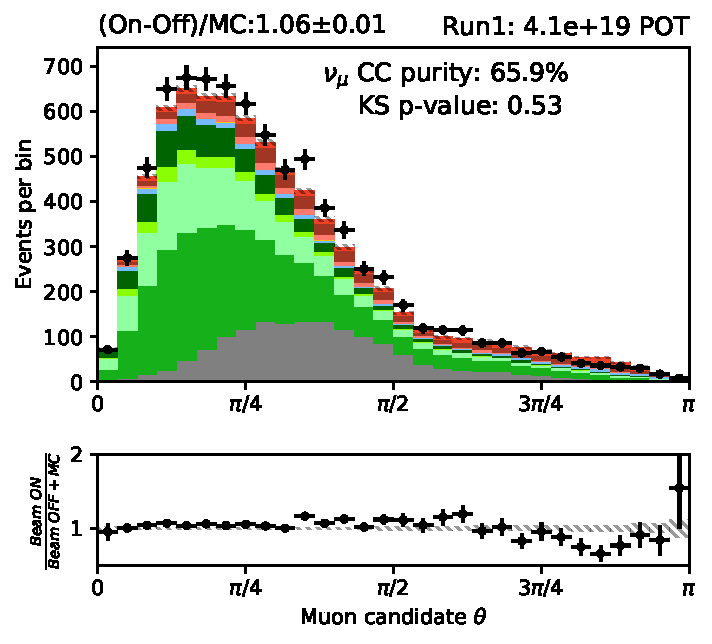
\includegraphics[height=4.25cm]{NuMuCCsel/Images/run1/numu_theta_run1.pdf}
    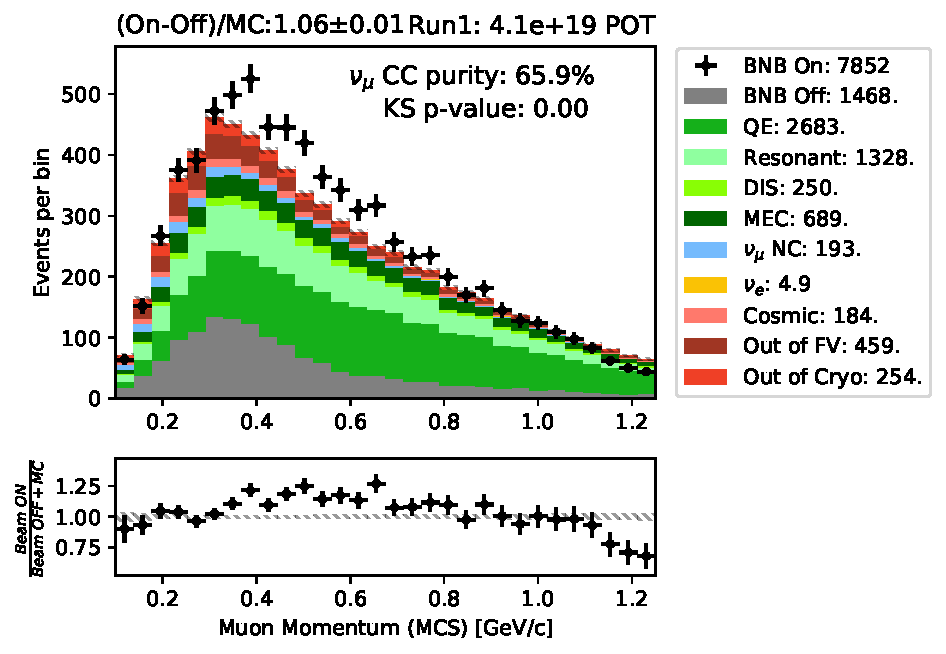
\includegraphics[height=4.25cm]{NuMuCCsel/Images/run1/numu_mcsmom_run1.pdf} \hspace{1mm}
    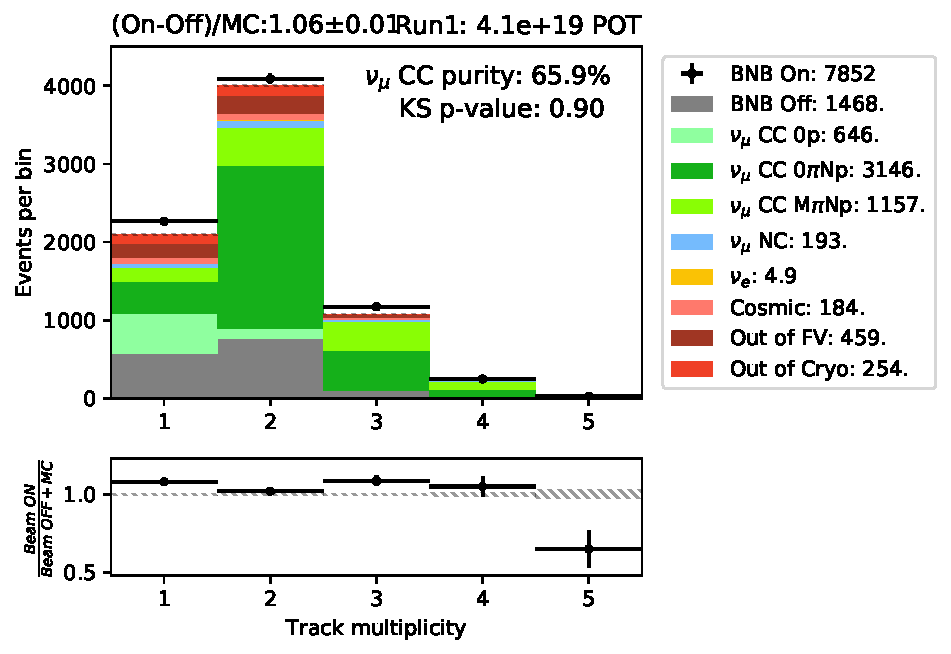
\includegraphics[height=4.25cm]{NuMuCCsel/Images/run1/numu_vtxntrack_cat_run1.pdf}
    \caption{(left) Kinematics of the muon tagged track. Because the selection is not contained, multiple coulomb scattering is used to determine the momentum. (right) Track multiplicity at vertex. An object is considered to be a track at vertex if the \textit{track\_score} $>$ 0.3 and \textit{trk\_distance} $<$ \SI{3}{\cm}.}
    \label{fig:numu:mcs}
\end{figure}

\begin{figure}[H]
    \centering
    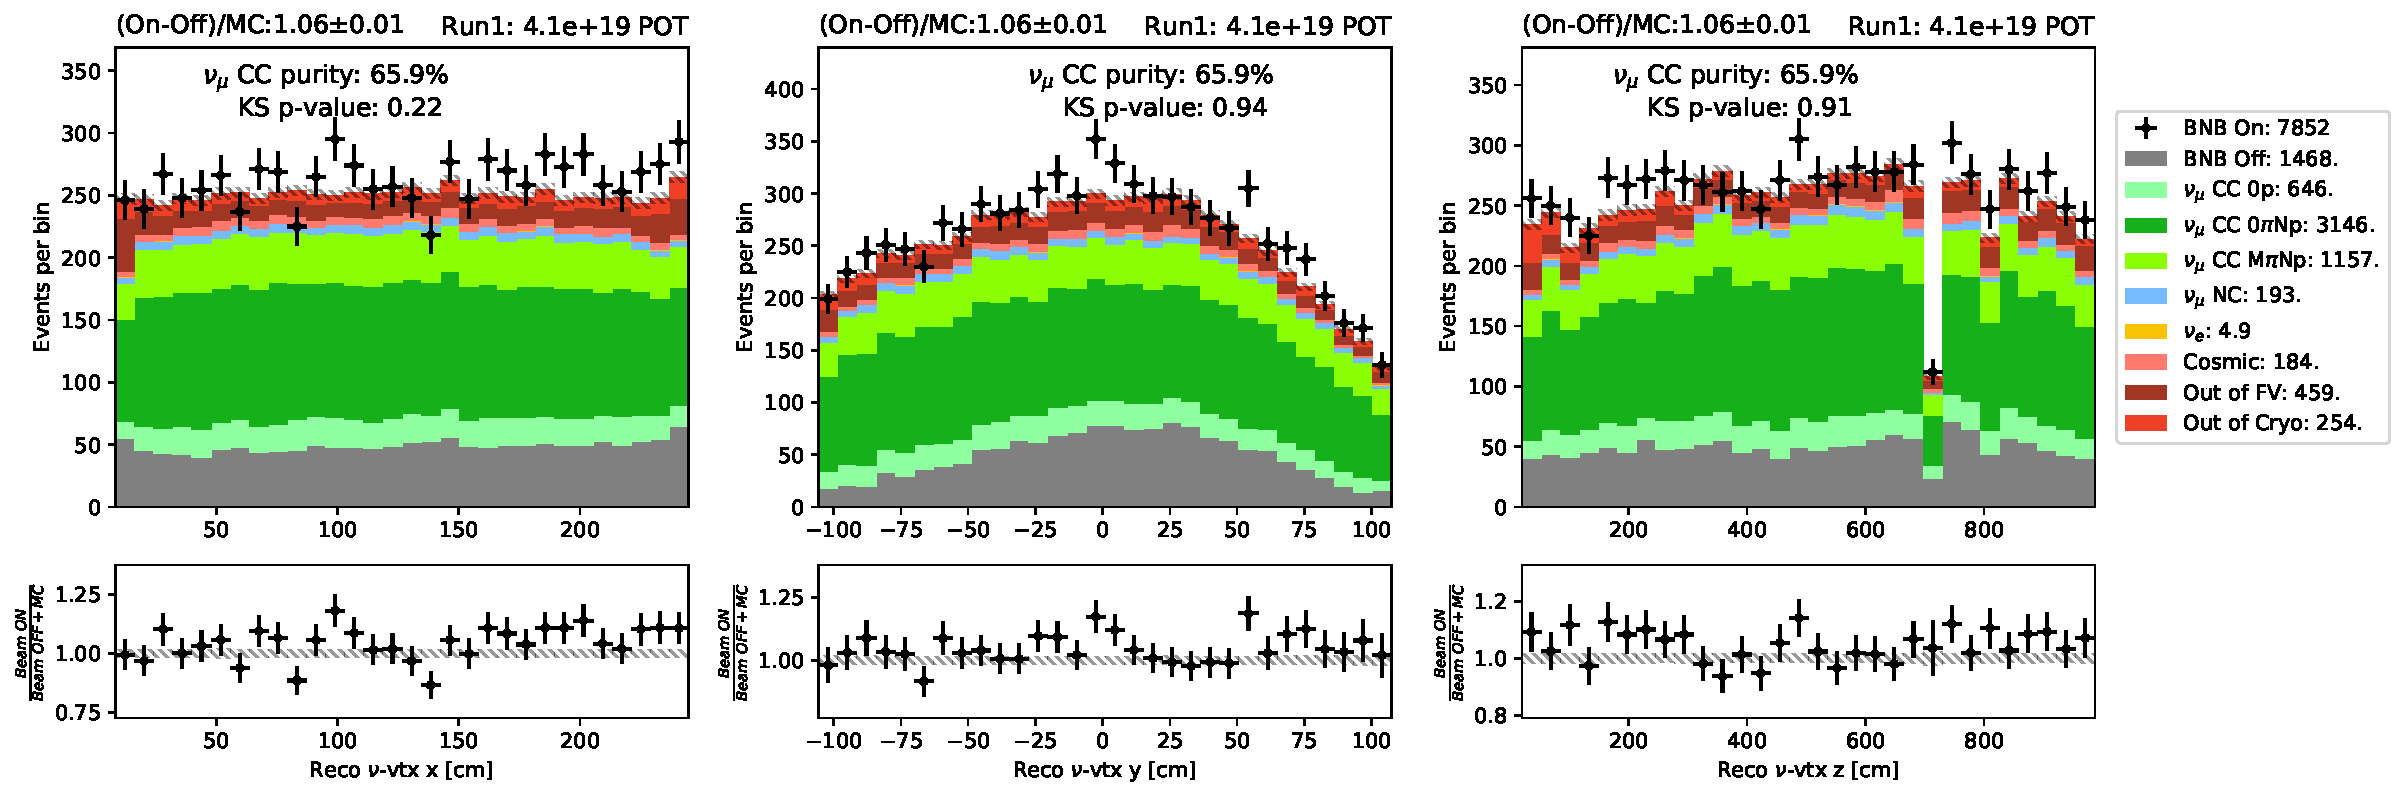
\includegraphics[height=5.35cm]{NuMuCCsel/Images/run1/numu_recovtx_run1.pdf}
    \caption{Position of the reconstructed vertex after the selection. Notice the high purity event at the edges of the detector. The reduced efficiency due to the dead wire region is clearly visible.. Because the purity is reasonable, it was chosen to be as inclusive as possible and not remove the region.}
    \label{fig:numu:vtx}
\end{figure}

\paragraph{High purity selection}
When using the Run3 open data, we can use the CRT to achieve higher a higher purity. Nonetheless, exiting muon tracks might trigger the CRT veto as well, therefore the higher purity selection includes both containment and CRT veto. The additional cuts are:
\begin{itemize}
    \item \textit{all\_end\_contained}
    \item \textit{CRT Veto} != 1 or \textit{crthitpe} $<$ 100
    \item \textit{closestNuCosmicDist} $>$ \SI{5}{\cm}
\end{itemize}
Due to the fact that most $\nu_\mu$ CC inclusive events are not contained, the efficiency drops to 17.5\%, see \cref{fig:numu:eff_r3}. Note that the denominator here still contains both contained and uncontained events to enable comparison with the previous section. At the very lowest neutrino energies, below \SI{\approx 400}{\MeV}, the efficiency is only slightly reduced. The overall purity goes up to \SI{77.6}{\%}. 

\begin{figure}[H]
    \centering
    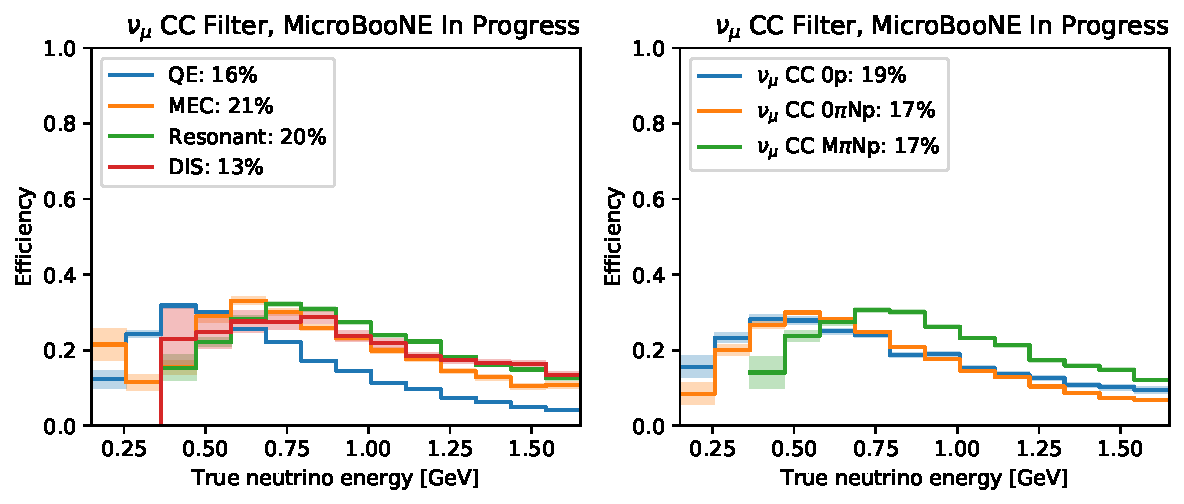
\includegraphics[width=0.65\textwidth]{NuMuCCsel/Images/run3/numu_efficiency_run3.pdf}
    \caption{Efficiency of the $\nu_\mu$ CC contained selection with CRT for different interaction categories (left) and final states (right) in function of the true neutrino energy.}
    \label{fig:numu:eff_r3}
\end{figure}

\paragraph{Energy reconstruction in the high-purity selection} 
In a contained selection, range based momentum can be used to estimate the energy. Therefore there are two methods shown in this section:
\begin{itemize}
    \item Calorimetric energy estimate: the calorimetric information of the collection plane is used. For showers, the energy of the hits is summed and corrected for a bias. For tracks, the energy is obtained by summing over the energy over the track segments by multiplying the pitch with the local $d$E/d$x$. The mass of the muon is added to the sum.
    \item The range based momentum estimate is used to for the track-like particles. The energy is calculated under the muon hypothesis for the muon candidate. If there are other muon-like particles in the event (as defined earlier in this section) their energy is added under the charged pion hypothesis. The energy of other track-like particles is added under the proton hypothesis. Finally, for shower-like particles, the calorimetric estimate is used.
\end{itemize}
Both methods are compared in \cref{fig:numu:energy,fig:numu:reso_e}. The range based energy estimation clearly has a smaller bias and smaller spread compared to the calorimetric-based estimate. This is one of the major advantages of a contained selection which will further be stressed in the next section.

\begin{figure}[H]
    \centering
    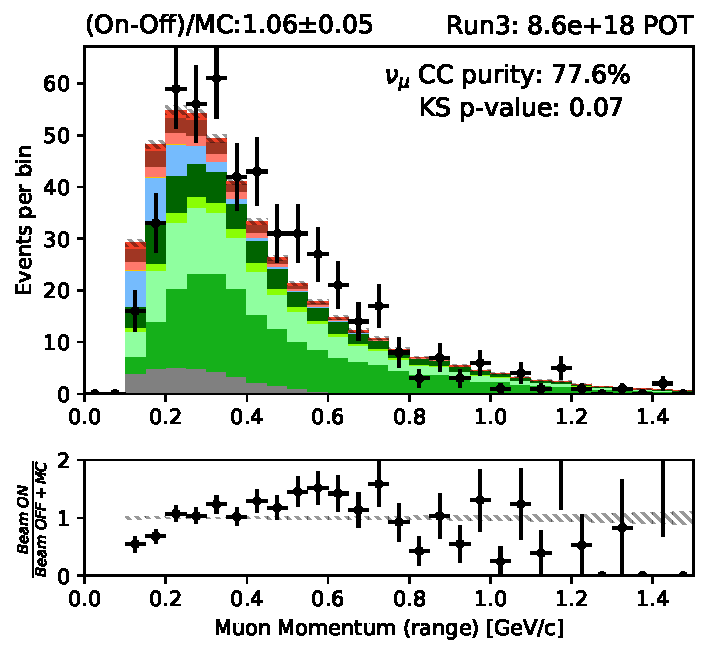
\includegraphics[height=4.35cm]{NuMuCCsel/Images/run3/numu_rangemom_run3} \hspace{2mm}
    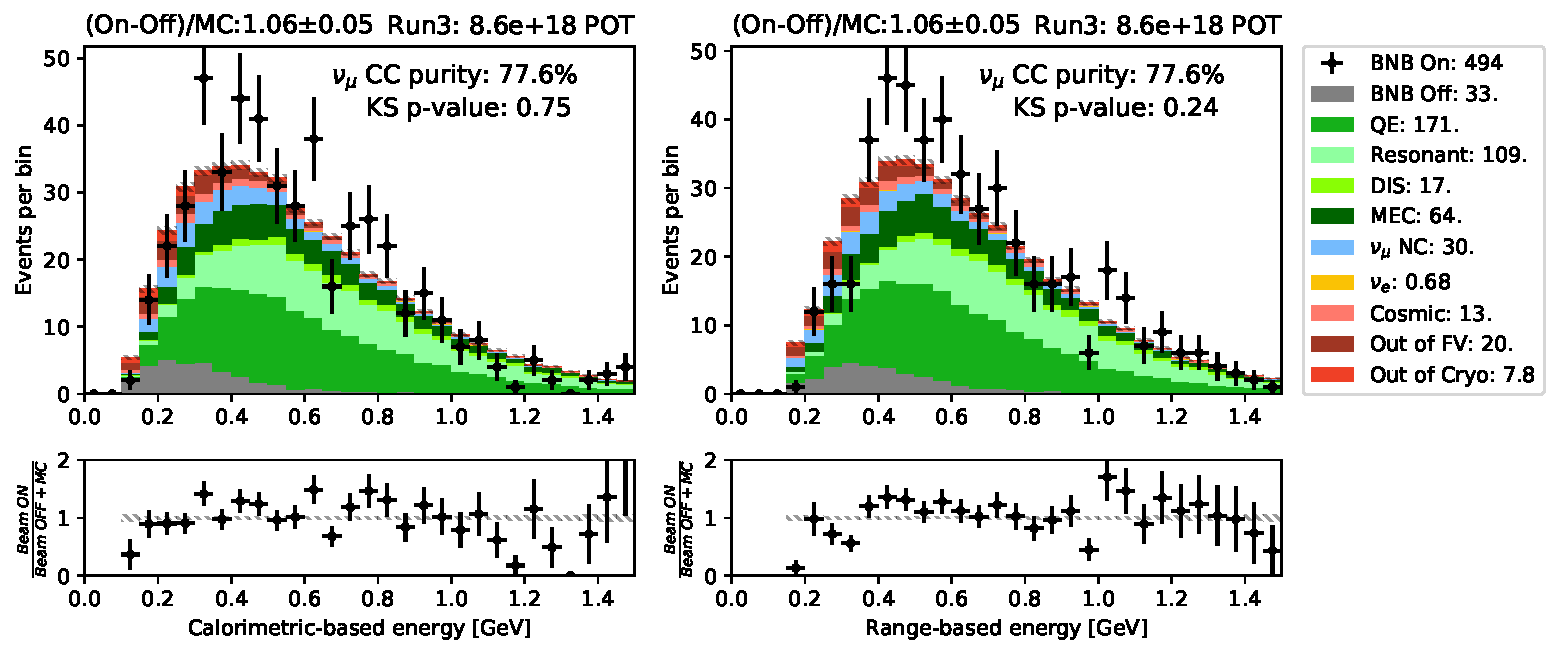
\includegraphics[height=4.35cm]{NuMuCCsel/Images/run3/numu_caloe_rangevscalo_run3.pdf}
    \caption{(left) Reconstructed muon momentum using the range-based estimation. Due to the \SI{10}{\cm} track-length requirement, there are no entries below \SI{0.11}{\GeV \per c}. (right) Reconstructed energy, both calorimetry-based and range-based, see text for details.}
    \label{fig:numu:energy}
\end{figure}

\begin{figure}[H]
  \begin{minipage}[c]{0.5\textwidth}
    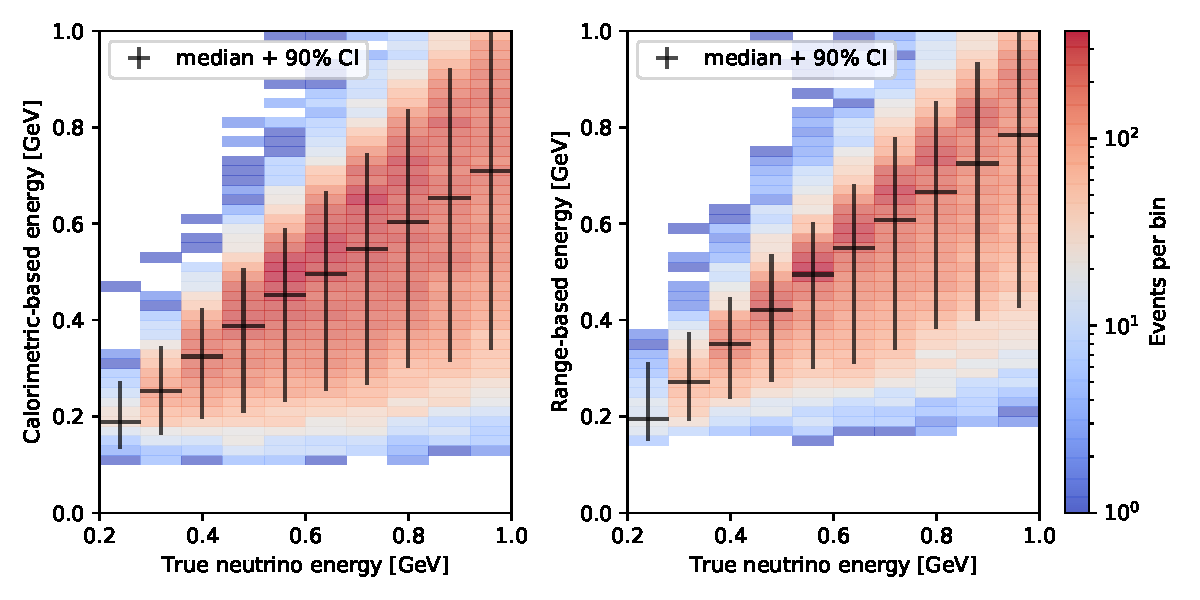
\includegraphics[width=\textwidth]{NuMuCCsel/Images/run3/resolution.pdf}
    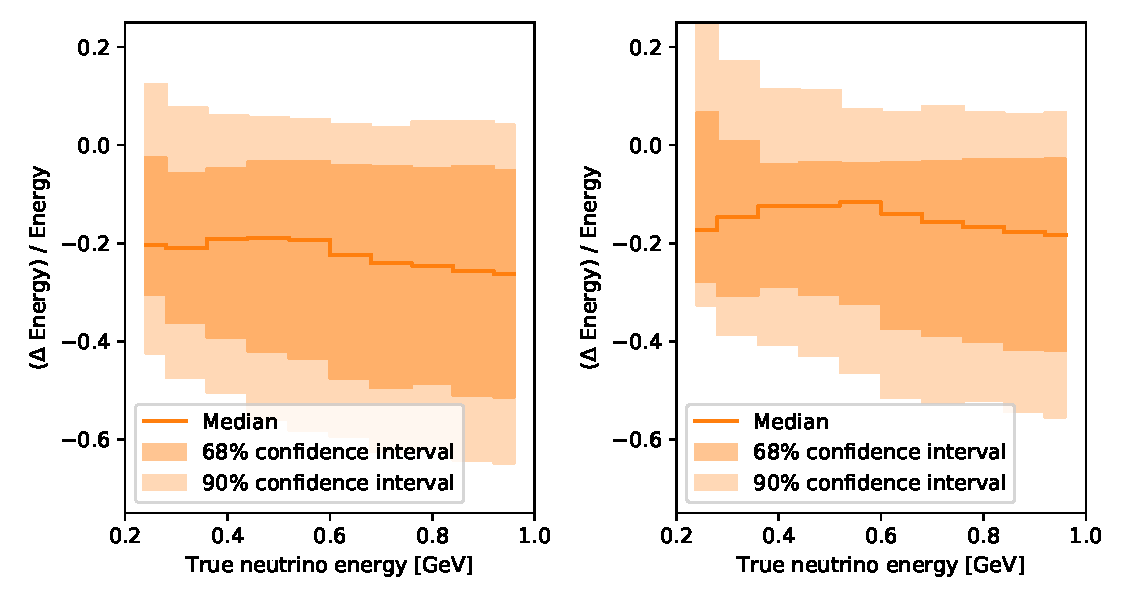
\includegraphics[width=0.88\textwidth]{NuMuCCsel/Images/run3/resolution_errors.pdf}
  \end{minipage}\hfill
  \begin{minipage}[c]{0.5\textwidth}
    \caption{
Comparison between the calorimetry-only (left panels) and the range-based (right panels) neutrino energy estimation. The top panel show the the reconstructed energy in function of the truth energy. In every bin, the black error bars correspond to the 5th, 50th and 95th percentile of the reconstructed energy distribution. The lower panel shows the fractional energy difference with 68\% and 90\% coverage intervals. 
    } 
    \label{fig:numu:reso_e}
  \end{minipage}
\end{figure}

\subsection{Constraint Selection \textcolor{red}{Ryan}}
\label{ssec:NuMUCCsel:constr}
\par The purpose of this $\nu_{\mu}$ side-band is to constrain the systematic uncertainties in the $\nu_{e}$ analysis. This is able to be done because the $\nu_{\mu}$s and $\nu_{e}$s of the BNB are subject to common, correlated uncertainties; the flux and cross-section models are discussed further in sec \ref{ssec:goalsofnumusel} and \ref{subsec:constraintfromnumu}. The $\nu_{e}$ selection is subject to higher uncertainties due to its low statistics. The $\nu_{\mu}$ channel benefits from two orders-of-magnitude larger absolute flux (Docdb 1031) therefore providing high-statistics samples which can be exploited to constrain the uncertainties on the $\nu_{e}$ predicted event rate. For more information regarding the philosophy and goals of this constraint see sec \ref{ssec:goalsofnumusel}.

\par This selection prioritizes higher efficiencies and purities in the low-energy region that is the interest to the LEE analysis. Unfortunately, the flux and cross-section predictions for $\nu_{e}$ are most uncertain in the few-hundreds MeV energy region. Fortunately, the absolute $\nu_{\mu}$ flux and the cross-species flux correlation is greatest below 1 GeV (see figs \ref{fig:numuconstraint:flux}, \ref{fig:numuconstraint}) where its constraining power is most needed.
\begin{comment}
\begin{figure}
    \centering
    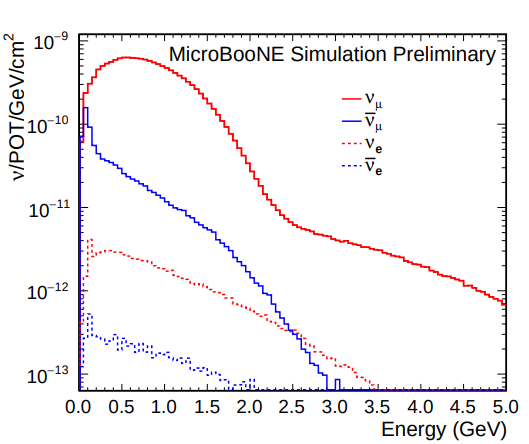
\includegraphics[height=6.5cm]{NuMuCCsel/Images/Ryan/absoluteFlux_uBooNE.png} \hspace{2mm}
    \caption{The absolute neutrino flux prediction through the MicroBooNE detector as calculated by the beam simulation. Shown is the flux for $\nu_{\mu}$, $\overline{\nu_{\mu}}$, $\nu_{e}$, and $\overline{\nu_{e}}$ averaged through the TPC volume with dimensions 2.56m by 2.33m by10.37m. DocDb 1031}
    \label{fig:bnb_absoluteflux}
\end{figure}
\end{comment}
\subsubsection{Signal Definition}
\label{sssec:NuMUCCsel:constr:signaldef}
\par A $\nu_{\mu}$ event is identified by the presence of one muon candidate originating from inside the fiducial volume of the detector. Additional tracks and showers may accompany the muon candidate; these assist in reconstruction and neutrino energy calculation but are not necessary in the inclusive selection. Future studies of the $\nu_{\mu}$ side-band may require the presence of proton candidates to further constrain interaction models.

\subsubsection{Event Preselection}
\label{sssec:NuMUCCsel:constr:preselec}

\par The selection of $\nu_{\mu}$ events is built from the groundwork of the SliceID tool (sec. \ref{sec:sliceID:SliceID}) and a combination of cuts on event-level and track-level observable values. The cuts described in this section are chosen to reduce cosmic and dirt backgrounds and select slices that are $\nu_{\mu}$-like. The methodology of this selection is similar to the selections in Sec. \ref{sec:nueselection} where first, the common SliceID filter is applied; next, event-level cuts are applied to select $\nu_{\mu}$-like events; finally, track-level cuts are applied to screen for muon-like candidates. The muon-candidate selection is described in sec \ref{sssec:NuMUCCsel:constr:muonsel}.

\par The requirement that the reconstructed vertex be contained inside the fiducial volume and that the slice have a sufficiently high topological score favor $\nu_{\mu}$ CC events and disfavor activity that is cosmogenic or dirt-like. Those cuts, specifically, are:

\textbf{Runs 1+3:}
\begin{itemize}
    \item \emph{nslice} = 1.
    \item \emph{n\_tracks\_contained} $>$= 1.
    \item \emph{reco\_nu\_vtx\_sce\_x} $\in$ [5,251] cm.
    \item \emph{reco\_nu\_vtx\_sce\_y} $\in$ [-110,110] cm.
    \item \emph{reco\_nu\_vtx\_sce\_z} $\in$ [20,986] cm.
    \item \emph{topological\_score} $>$ 0.06.
    \item \emph{reco\_nu\_vtx\_sce\_z} $\not\in$ [675,775] cm.
\end{itemize}

\par \noindent The final cut on the $z$ coordinate is to eliminate events that exist in the region of `dead wires' in the MicroBooNE detector, this is common practice within the collaboration.

\par \noindent Run 3 has the additional power to leverage the CRT system to further limit cosmic contamination in the signal. Given that this selection targets contained events, the fact that $\nu_{\mu}$ interactions can lead to hits in the CRT does not hamper the analysis' performance.

\textbf{Run 3 only:}
\begin{itemize}
    \item \emph{CRT Veto} != 1 or \emph{crthitpe} $<$ 100
    \item \emph{closestNuCosmicDist} $>$ 5 cm
\end{itemize}

\subsubsection{Muon Selection}
\label{sssec:NuMUCCsel:constr:muonsel}

\par After the event-level cuts are applied, the tracks in the slice are further analyzed to identify muon candidates. At least one reconstructed track in the event must satisfy all these criteria for the event to pass the selection. If more than one track passes this requirement, then the longest is taken as the muon candidate. Of the muon candidates that pass this selection, $\approx 94\%$ are, in simulation, correctly tagged muons from $\nu_{\mu}$ CC interactions.

\begin{itemize}
    \item \emph{trk\_sce\_start\_x} $\in$ [5,251] cm.
    \item \emph{trk\_sce\_start\_y} $\in$ [-110,110] cm.
    \item \emph{trk\_sce\_start\_z} $\in$ [20,986] cm.
    \item \emph{trk\_sce\_end\_x} $\in$ [5,251] cm.
    \item \emph{trk\_sce\_end\_y} $\in$ [-110,110] cm.
    \item \emph{trk\_sce\_end\_z} $\in$ [20,986] cm.
    \item \emph{trk\_llr\_pid\_score} $>$ 0.2.
    \item \emph{trk\_trk\_score} $>$ 0.8.
    \item \emph{trk\_trk\_length} $>$ 10 cm.
    \item \emph{trk\_distance} $<$ 4 cm.
    \item \emph{pfp\_generation} = 2.
\end{itemize}

\par \noindent The cuts made on the start and end points of the reconstructed tracks require that the track is fully contained inside the fiducial volume of the detector. This containment cut further reduces the primary background for this selection are is cosmic muons, originating from outside the detector. The containment requirement also motivates the use of range-based momentum calculations on all the muon candidates. Range-based momentum has been shown to have a high resolution. \emph{Consistency between range-based and the independently calculated MCS-based momentum will be used in a future iteration of this analysis as an additional handle to increase purity (see figs \ref{fig:numusel:momres} and \ref{fig:NuMUCCsel:ryan:PQuality})}. The containment condition rejects many higher-energy $\nu_{\mu}$ events that might leave the detector, but it has a high efficiency in the lower energies.

\par The cut on the $trk_distance$ requires that the reconstructed track be sufficiently close to the interaction vertex, this removes many in-time cosmic muons that are reconstructed as part of the event.

\par The cut on the log likelihood ratio pid score is to separate the muons from the protons among the PFParticle tracks in the passing slices. The track length cut further separates the muons from the protons which tend to have shorter track lengths. 

\par The track score cut ensures that the selected tracks are particularly track-like and this removes many \textcolor{red}{particularly high energy (unclear why this is the case)}, track-like showers from the selection. Finally the PFParticle generation cut ensures that Pandora recognizes that the track is produced directly at the neutrino interaction vertex, and not as a secondary particle (i.e. in a $\pi \rightarrow \mu$ decay or re-interaction). 

\begin{figure}
    \centering
    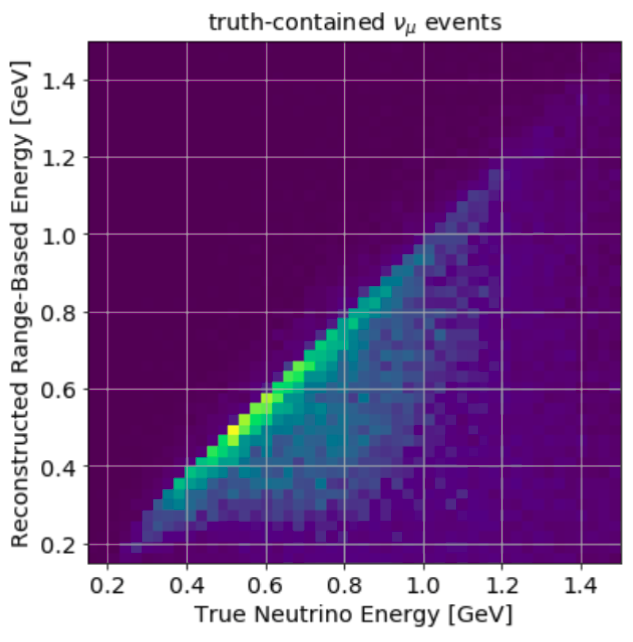
\includegraphics[height=6.5cm]{NuMuCCsel/Images/Ryan/containedMomentumRes.png} \hspace{2mm}
    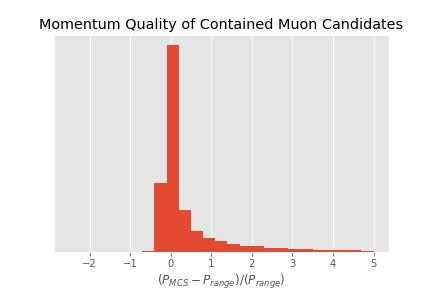
\includegraphics[height=6.5cm]{NuMuCCsel/Images/Ryan/muoncandidate_pquality.jpg} \hspace{2mm}
    \caption{The performance of range-based $\mu$ momentum calculation for contained tracks.}
    \label{fig:numusel:momres}
\end{figure}

\begin{figure}[ht] 
\begin{center}
    \begin{subfigure}[b]{0.45\textwidth}
    \centering
    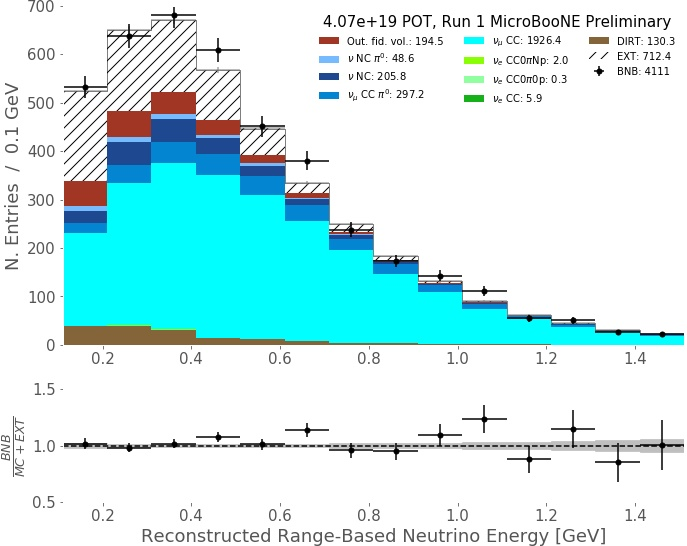
\includegraphics[width=1.00\textwidth]{NuMuCCsel/Images/Ryan/Run1_recoErange_FullSel.jpg}
    \caption{\label{fig:NuMUCCsel:ryan:noPQuality} After full selection.}
    \end{subfigure}
    \begin{subfigure}[b]{0.45\textwidth}
    \centering
    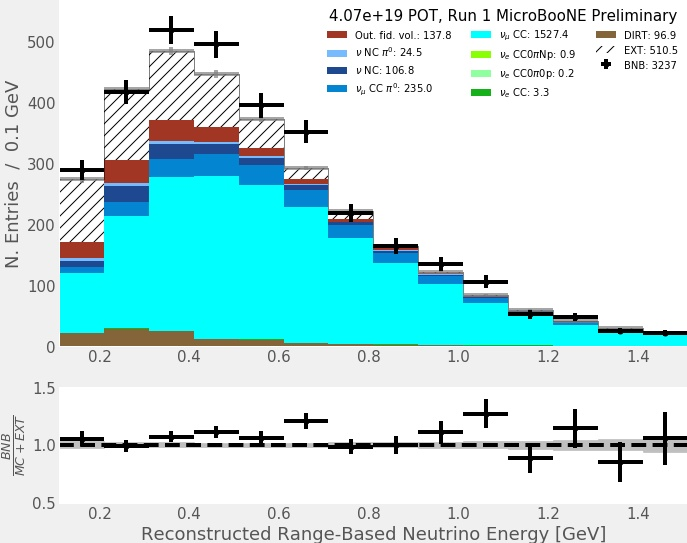
\includegraphics[width=1.00\textwidth]{NuMuCCsel/Images/Ryan/Run1_recoErange_pquality.jpg}
    \caption{\label{fig:NuMUCCsel:ryan:withPQuality} After full selection and momentum quality cut.}
    \end{subfigure}
\caption{The distribution of range-based energy calculations for each passing slice. Fig \ref{fig:NuMUCCsel:ryan:withPQuality} shows the distribution after a quality cut, keeping events that fall within 0.5 of the peak in the right plot of fig \ref{fig:numusel:momres}.}
\label{fig:NuMUCCsel:ryan:PQuality}
\end{center}
\end{figure}


\subsubsection{Determination of Fiducial Volume}
\label{sssec:NuMUCCsel:constr:FV}

\par This selection leverages the availability of a fully calibrated E-field map to perform space-charge corrections on the start and end-points of reconstructed tracks. This allows to impose a tight fiducial volume which maximizes the selection efficiency without impacting reconstruction performance. The fiducial volume is defined to be: 

\begin{itemize}
    \item x $\in$ [5,251]
    \item y $\in$ [-110,110]
    \item z $\in$ [20,986]
\end{itemize}

\begin{comment}
\par The fiducial volume in this section differs slightly from other fiducial volumes, even in this analysis. Because the purpose of this selection is to leverage the high-statistics of the $\nu_{\mu}$ composition of the BNB, the fiducial volume is taken to be as large as possible while retaining high purity and efficiency at low-energies.

\par With the exception of the downstream fiducial volume face, all the fiducial volume boundaries are chosen in order to retain as many signal events as possible. The SCE-correction procedure is quite effective and can recover the true value give or take a few centimeters, with slightly less resolution near the boundaries. The resolution is shown in fig \ref{fig:NuMUCCsel:ryan:sceres_y} for the x-direction; the performance is similar in the x, y, and z directions. See fig \ref{fig:NuMUCCsel:ryan:FVhighy} for an example of signal purity near a boundary using the spacecharge-corrected coordinates. Together, the spacecharge boundary that was found to maintain the highest purity is defined by


\begin{figure}
    \centering
    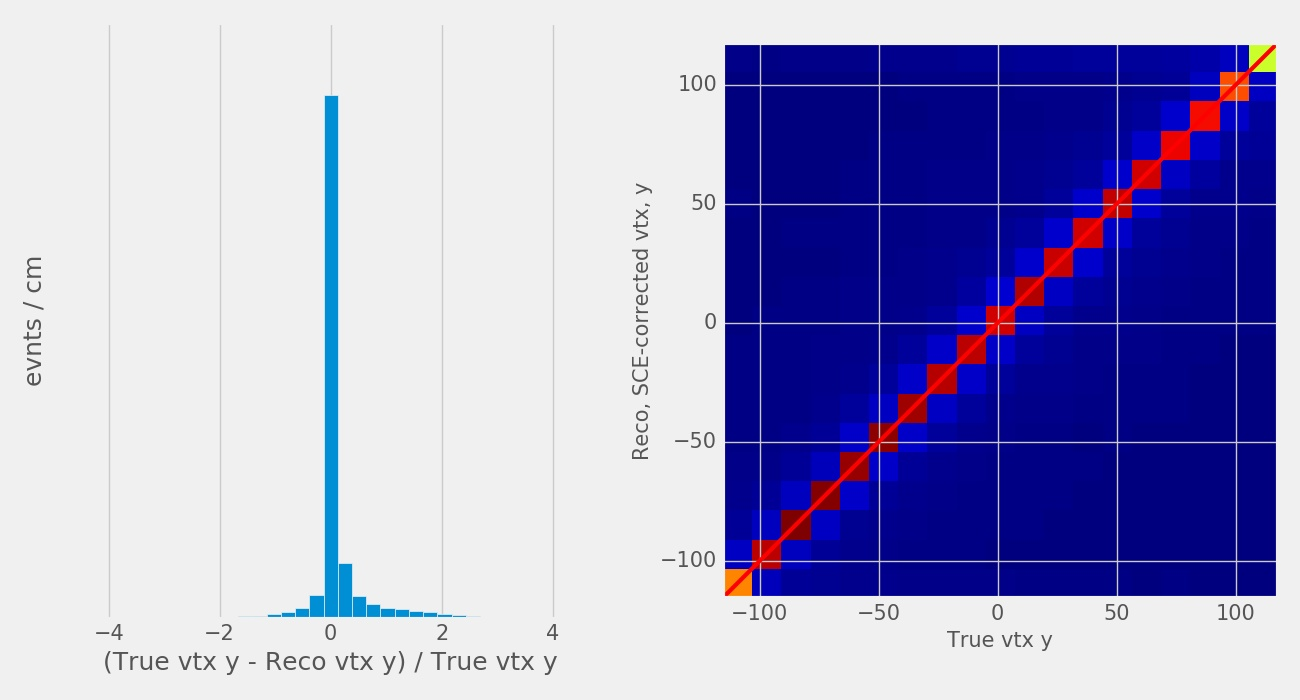
\includegraphics[height=6.5cm]{NuMuCCsel/Images/Ryan/sceresolution_y.jpg} \hspace{2mm}
    \caption{Resolution of the spacecharge-corrected vertex positions. The spacehcarge-corrected y-coordinates are being compared to the truth values without spacecharge distortion. }
    \label{fig:NuMUCCsel:ryan:sceres_y}
\end{figure}

\begin{figure}[ht] 
\begin{center}
    \begin{subfigure}[b]{0.45\textwidth}
    \centering
    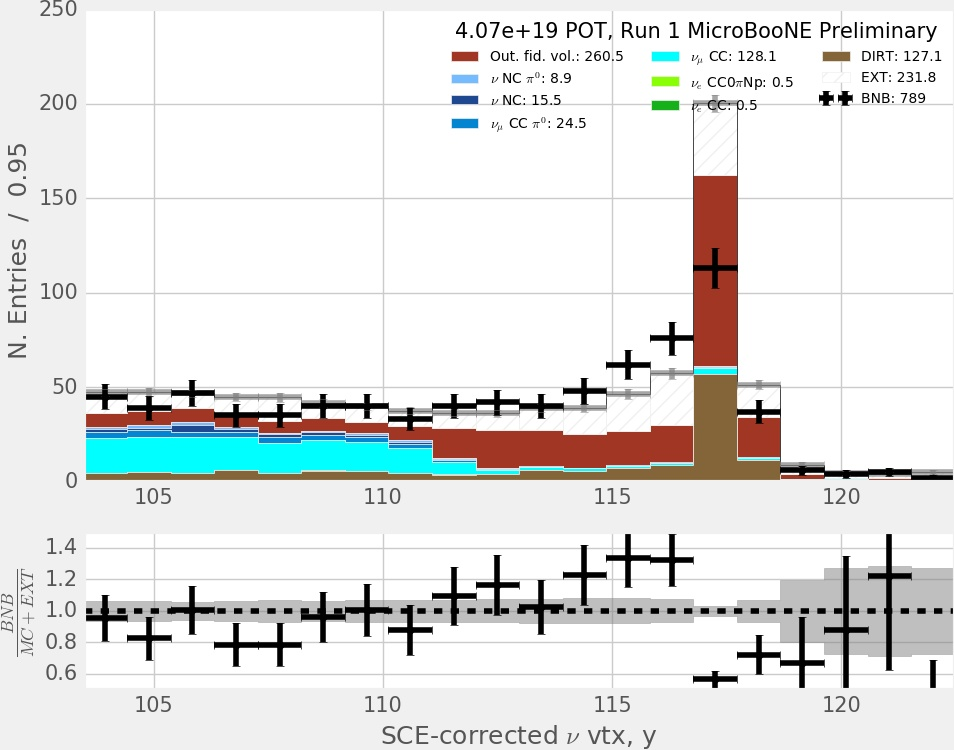
\includegraphics[width=1.00\textwidth]{NuMuCCsel/Images/Ryan/Run3_MCData_highy.jpg}
    \caption{\label{fig:NuMUCCsel:ryan:FVhighyMC} Data-MC distribution near top of detector.}
    \end{subfigure}
    \begin{subfigure}[b]{0.45\textwidth}
    \centering
    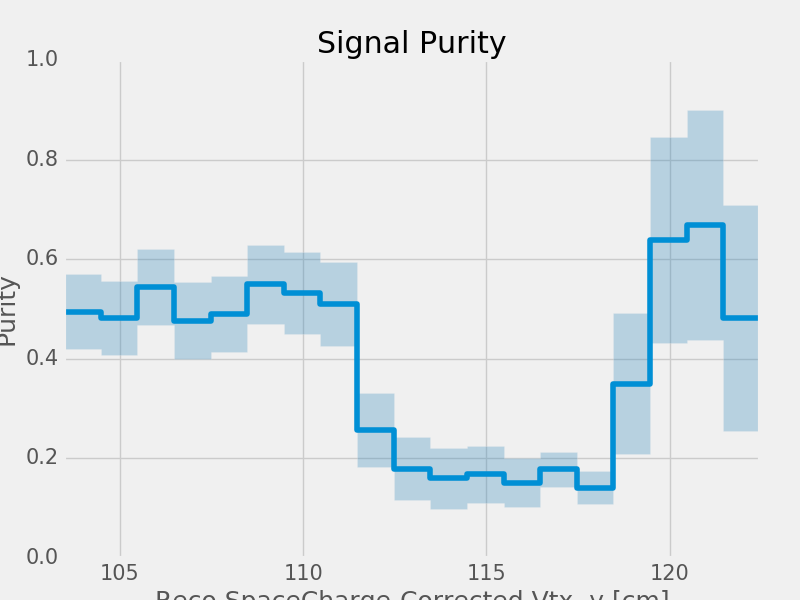
\includegraphics[width=1.00\textwidth]{NuMuCCsel/Images/Ryan/SignalPurity_highy.png}
    \caption{\label{fig:NuMUCCsel:ryan:FVhighyPur} Signal Purity}
    \end{subfigure}
\caption{Example of signal composition near boundary.}
\label{fig:NuMUCCsel:ryan:FVhighy}
\end{center}
\end{figure}
\end{comment}

\subsubsection{Performance}
\label{sssec:NuMUCCsel:constr:performance}

\par This selection has been evaluated on the Run1 and the Run3 open datasets processed for this analysis. The advantage of the Run 1 data-set is higher statistics ($4E19$ POT in Run1 and $0.9E19$ POT in Run3). Run 3 allows to use the CRT system for extra background rejection. Distributions shown in this section will be of variables pertaining to the muon candidate for each event that passes the selection; Run1 data will be preferentially shown due to the higher statistics. The power of the Run3 CRT system will be demonstrated at the end of this section.

\par Run 3 data includes information from the CRT system which was unavailable for the first MicroBooNE run. See fig \ref{fig:NuMUCCsel:ryan:Run3CRTcomp} for an example of the impact of the CRT. The CRT veto will eliminate more than 70$\%$ of the cosmics while suffering only roughly 15$\%$ loss in signal.

\par The overall efficiency of this selection is \textcolor{pink}{finish remaking these plots with newest data} ???$\%$ and overall purity is ???$\%$. The priority of the selection was to maximize purity and efficiency in the low-energy region (see fig ???). The effectiveness of this selection can not by explained by distributions, efficiencies, and purities alone; it relies on the constraining power. See sec \ref{ssec:finalSensitivityCalc} for a technical discussion of the incorporation of this selection into the final analysis sensitivity.

\begin{figure}[H] 
\begin{center}
    \begin{subfigure}[b]{0.3\textwidth}
    \centering
    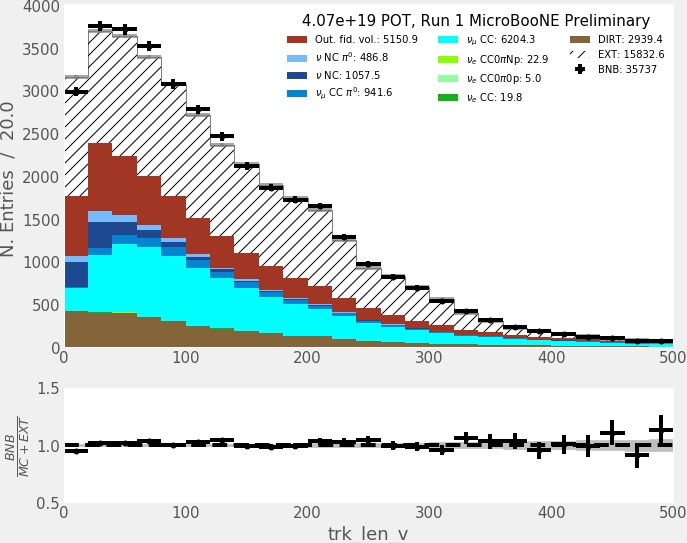
\includegraphics[width=1.00\textwidth]{NuMuCCsel/Images/Ryan/Run1_trklen_justSlice.jpg}
    \caption{\label{fig:NuMUCCsel:ryan:trklenSliceID} after SliceID}
    \end{subfigure}
    \begin{subfigure}[b]{0.3\textwidth}
    \centering
    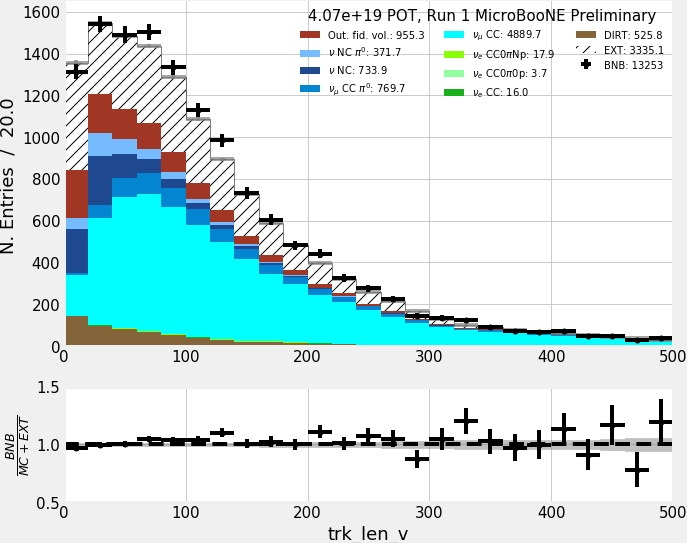
\includegraphics[width=1.00\textwidth]{NuMuCCsel/Images/Ryan/Run1_trklen_justEvtsel.jpg}
    \caption{\label{fig:NuMUCCsel:ryan:trklenEvt} after event-level preselection}
    \end{subfigure} %\newline
    \begin{subfigure}[b]{0.3\textwidth}
    \centering
    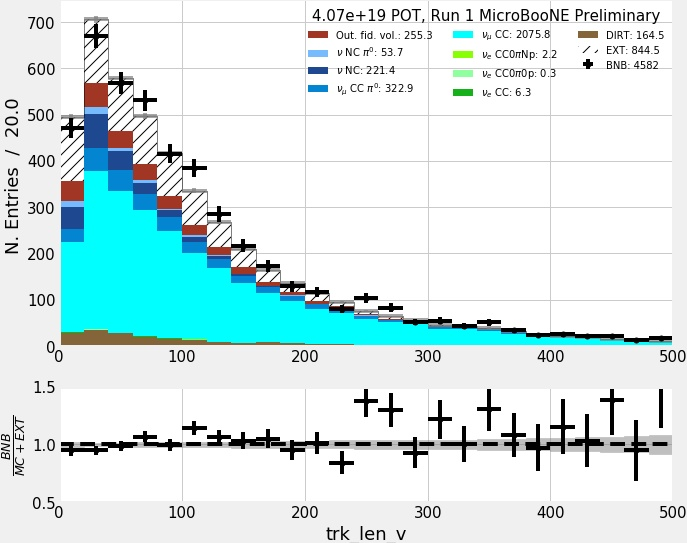
\includegraphics[width=1.00\textwidth]{NuMuCCsel/Images/Ryan/Run1_trklen_fullSel.jpg}
    \caption{\label{fig:NuMUCCsel:ryan:trklenFull}  With muon-tagging}
    \end{subfigure}
\caption{Track length of muon candidates. Just statistical uncertainties shown.}
\end{center}
\end{figure}

\begin{figure}[H] 
\begin{center}
    \begin{subfigure}[b]{0.3\textwidth}
    \centering
    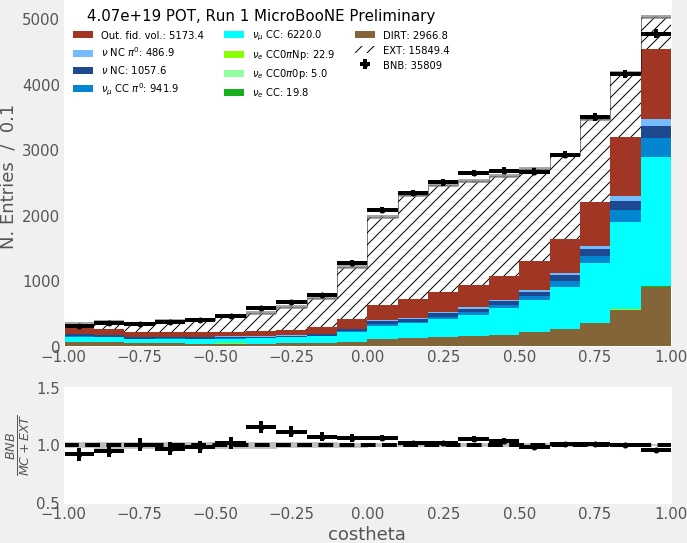
\includegraphics[width=1.00\textwidth]{NuMuCCsel/Images/Ryan/Run1_costheta_justSlice.jpg}
    \caption{\label{fig:NuMUCCsel:ryan:trklenSliceID} after SliceID}
    \end{subfigure}
    \begin{subfigure}[b]{0.3\textwidth}
    \centering
    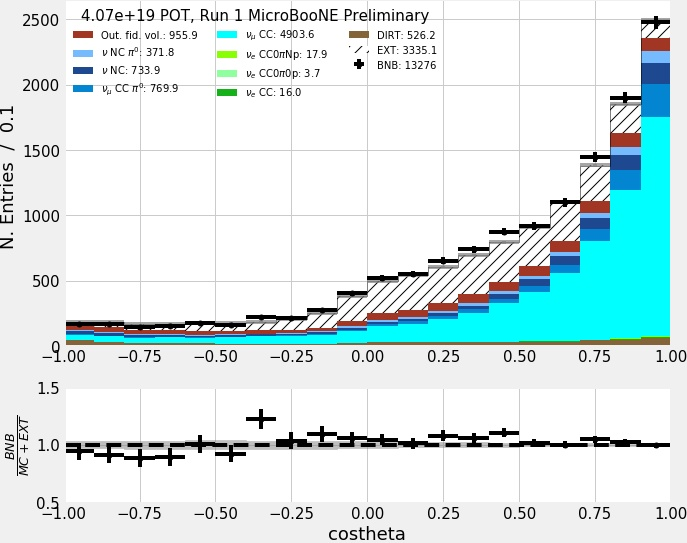
\includegraphics[width=1.00\textwidth]{NuMuCCsel/Images/Ryan/Run1_costheta_justEvtsel.jpg}
    \caption{\label{fig:NuMUCCsel:ryan:trklenEvt} after event-level preselection}
    \end{subfigure} %\newline
    \begin{subfigure}[b]{0.3\textwidth}
    \centering
    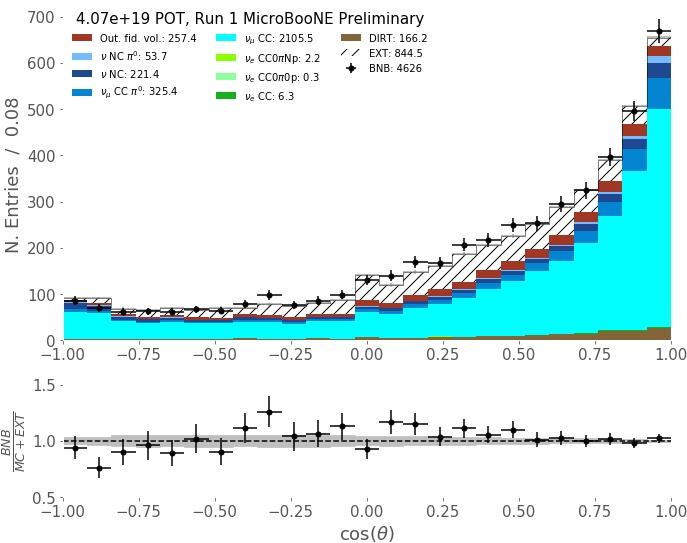
\includegraphics[width=1.00\textwidth]{NuMuCCsel/Images/Ryan/Run1_costheta_fullSel.jpg}
    \caption{\label{fig:NuMUCCsel:ryan:trklenFull} With muon-tagging}
    \end{subfigure}
\caption{Cosine of the track angle of muon candidates with respect to the beam-direction. Just statistical uncertainties shown.}
\end{center}
\end{figure}

\begin{figure}[ht] 
\begin{center}
    \begin{subfigure}[b]{0.45\textwidth}
    \centering
    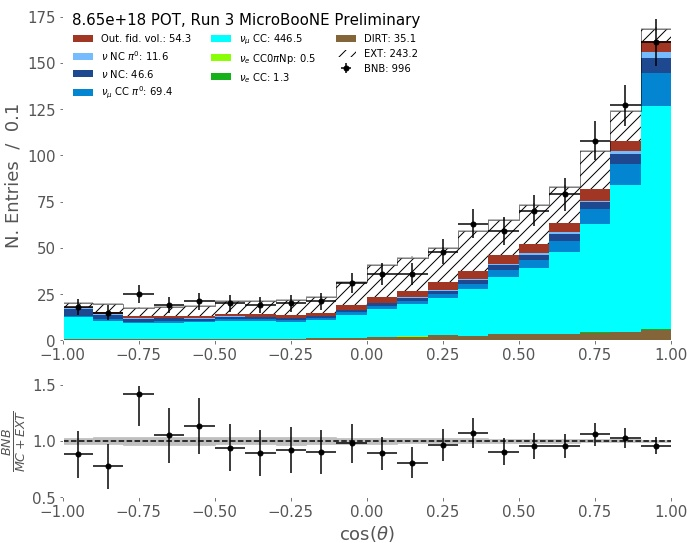
\includegraphics[width=1.00\textwidth]{NuMuCCsel/Images/Ryan/Run3_costheta_noCRT.jpg}
    \caption{\label{fig:NuMUCCsel:ryan:coswithCRT} without CRT}
    \end{subfigure}
    \begin{subfigure}[b]{0.45\textwidth}
    \centering
    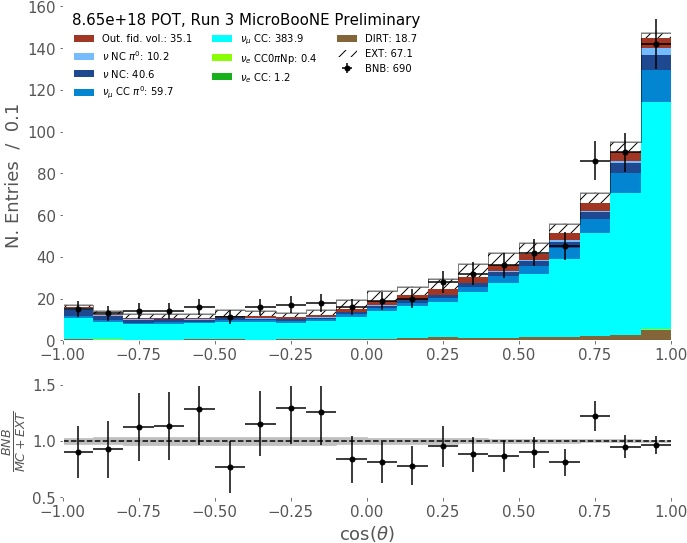
\includegraphics[width=1.00\textwidth]{NuMuCCsel/Images/Ryan/Run3_costheta_withCRT.jpg}
    \caption{\label{fig:NuMUCCsel:ryan:cosnoCRT} with CRT veto}
    \end{subfigure}
\caption{Angle with respect to the beam-direction of muon candidates for $\nu_{\mu}$ constraint. Just statistical uncertainties shown.}
\label{fig:NuMUCCsel:ryan:Run3CRTcomp}
\end{center}
\end{figure}

\textcolor{red}{Missing data-mc plot of reconstructed range-based neutrino energy.}

\textcolor{blue}{The selection described in this section shows a good level of data-simulation agreement for both Run 1 and Run 3, and is highly enriched in $\nu_{\mu}$ events which are reconstructed with very good energy resolution. \emph{Events from this selection are to be used to constrain $\nu_e$ flux and cross-section modeling uncertainties. While this excercise has not been fully performed at the current time, it is expected to be completed by the Feb. 2020 collaboration meeting.}}
